\documentclass[ fontsize=11pt]{article}
\linespread{1.5}
% \usepackage[margin=2.5cm]{geometry}
\usepackage[margin=2.5cm, headheight=0pt, headsep=1cm]{geometry}
\usepackage{enumerate, fancyhdr, graphicx, amsmath, float}
\usepackage{hyperref}


\title{Old School \tetris{} Meets Page Rank}
\author{Paul Chesnais (pmc85) and Sam Svenningsen (sjs382)}
\date{}

\def\tetris{Tetris\textsuperscript{\textregistered}}

\pagestyle{fancy}
\fancyhead{}
\lhead{pmc85 and sjs382}
\chead{Old School \tetris{} Meets Machine Learning}
\rhead{\today}
\fancyfoot{}
\rfoot{\thepage}
\lfoot{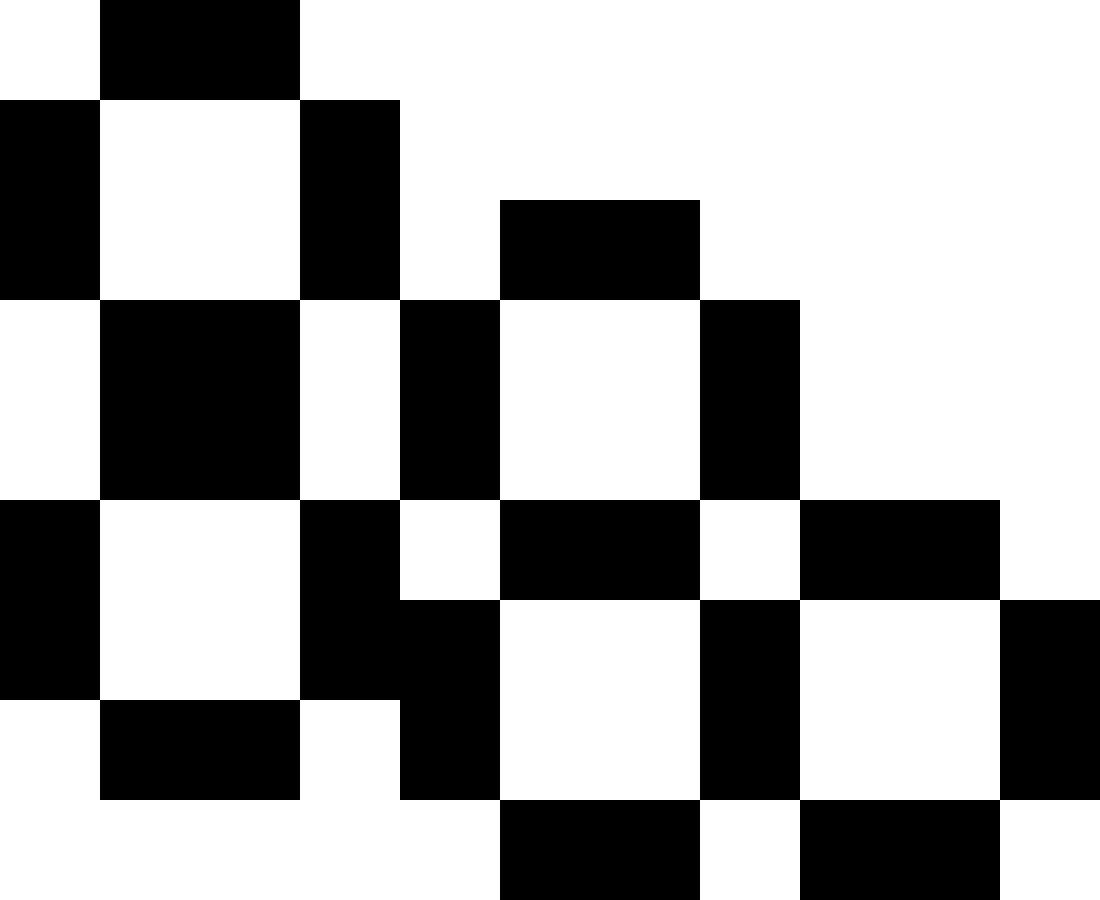
\includegraphics[height=20pt]{Logo}}
\renewcommand{\headrulewidth}{0.5pt}
\renewcommand{\footrulewidth}{0.5pt}


\begin{document}
\maketitle
\thispagestyle{empty}
\figure{\center{
\includegraphics[height=125pt]{tetris}}}
\figure{\center{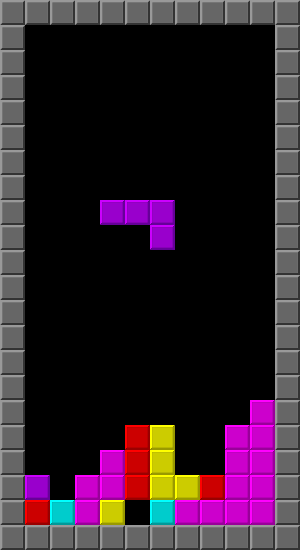
\includegraphics[height=300pt]{tetris_screen}}}
\newpage
\section{Abstract}
\label{sec:abstract}

\par We built a \tetris{} bot that plays \tetris{}, the Russian tile-matching puzzle video game. It has been shown that \tetris{} is NP-C \cite{tetrishard}, so none of our solutions are, or can be (assuming $P \neq NP$), perfect.  We solved it by simplifying the contour (of the top of the \tetris{} blocks on the board) into a sequence of incremental changes in height going left to right. We then can compute the rank of all possible contours iteratively, and rank them.




\section{Motivation}
\label{sec:motivation}
One of us is a super \tetris{}fan


\section{Initial Attempts}
\label{sec:initial_attempts}

\section{Challenges Faced}
\label{sec:challenges_faced}

\par Scala optimization


\section{Current Version}
\label{sec:current_version}

\section{Conclusion}
\label{sec:conclusion}

\newpage


\begin{thebibliography}{9}
\bibitem{tetrishard}
Erik D. Demaine, Susan Hohenberger, David Liben-Nowell
\textit{
Tetris is Hard, Even to Approximate}.
\\\href{https://arxiv.org/abs/cs/0210020}{arXiv:cs/0210020}

\end{thebibliography}


\end{document}
